\documentclass[10pt,a4paper,openany]{book}
\usepackage[francais]{babel}

\usepackage[utf8]{inputenc}
\usepackage[a4paper]{geometry}
\usepackage[T1]{fontenc}
\usepackage{titling}
%\usepackage{showframe}
\usepackage{graphicx}

\usepackage{tcolorbox}
\tcbuselibrary{skins}
\newtcolorbox{warning}{colback=red!5!white, colframe=red!75!black, fonttitle=\bfseries, title=Attention !}
\newtcolorbox{notice}{colback=blue!5!white, colframe=blue!75!black, fonttitle=\bfseries, title=Notice}

\usepackage{listings, multicol, color, fancyhdr,lastpage}
\usepackage[font=small,format=plain,labelfont=bf,up,textfont=it,up]{caption}
\usepackage[hyperindex=true,colorlinks=true,breaklinks=true,linkcolor=blue]{hyperref}

\usepackage[font={large,itshape}]{quoting}

\pagestyle{fancy}
\fancyhead[LE,RO]{\leftmark}
\fancyhead[LO,RE]{}

\lstset{
	language=bash,						% le language par défaut
	title=\lstname,						% on donne le nom des fichiers inclus
	basicstyle=\ttfamily\normalsize,	% la fonte de base: brute d'imprimerie
	frame=leftline,	% une ligne à gauche
	rulecolor=\color{black},	% if not set, the frame-color may be changed on line-breaks within not-black text (e.g. commens (green here))
	framerule=2pt,
	%framexleftmargin=10pt,
	keywordstyle=\color{blue},	% keyword style
	commentstyle=\color{gray},	% comment style
	stringstyle=\color{mauve},	% string literal style
	escapeinside={\%*}{*)},		% if you want to add a comment within your code
	morekeywords={*,...},		% if you want to add more keywords to the set
	morecomment=[l]{\#},
	belowskip=10pt,
	aboveskip=0pt,
	xleftmargin=25pt,
	belowcaptionskip=0pt,
	abovecaptionskip=0pt
	}

\definecolor{dkgreen}{rgb}{0,0.6,0}
\definecolor{gray}{rgb}{0.5,0.5,0.5}
\definecolor{mauve}{rgb}{0.58,0,0.82}

% fonte
\renewcommand{\familydefault}{\sfdefault}
\renewcommand{\labelitemi}{$\bullet$}


\title{\huge\bsc{Des chiffres et des lettres}}
\author{Stéphane \bsc{22Decembre Guedon}}
\date{13 mai 2015}

\pretitle{\begin{center}}
	
\posttitle{
	\newline
		\Large\emph{Protéger ses communications en ligne\\et autres aspects de sa vie numérique\\}
		\vspace{5mm}
		\LARGE\emph{GnuPG et OpenPGP pour tous\\}
	\end{center}
		}

\preauthor{\centering
	    \vspace{5mm}
		
\includegraphics[width=0.9\textwidth]{./images/logo-gnupg}
		\vspace{1cm}
		\newline
	}

\postauthor{
	 \vspace{5mm}\\
		}

\predate{\begin{center} version 1 du }
	
	
\postdate{\end{center}}
	

\begin{document}
	%\makeatletter
	\maketitle

	%\frontmatter
	\chapter{Préambule}
	
	Ce document utilise les textes issus du tutoriel ou how-to GPG que j'ai écris. Il s'agit là de la version \textit{de base}, soit les fonctions que j'estime les plus importantes de GnuPG et OpenPG.
	
	Ce How-to peut être lu sur mon site internet\footnote{version anglaise: \url{http://www.22decembre.eu/category/howto-gpg.html}. Cliquez sur les liens «fr» sous les titres pour lire les articles en français.} Je vous encourage vivement à le partager, le repartager, que ce soit pour la version en ligne (html) ou hors-ligne (le pdf que vous êtes en train de lire).
	
	Bien entendu, les textes ont été légèrement modifiés pour correspondre à la forme qui lui est donné ici, à savoir un mini livre.
	
	Le but avoué de ce document est d'encourager les utilisateurs d'internet, soit en fait une grosse partie de la population occidentale, à protéger leurs communications telles que courriels et messagerie instantanée.
	
	Au moment même de la rédaction de ce livre, une loi extrêmement dangereuse pour les libertés 
	civiles est en cours d'adoption par le parlement et le gouvernement français.\footnote{\url{http://www.senat.fr/espace_presse/actualites/201505/un_projet_de_loi_pour_renforcer_les_services_de_renseignement.html}}
	
	Le fichier support à ce document, à savoir le fichier pdf que vous lisez, est signé avec ma clé gpg ainsi que la clé gpg créée exprès pour les besoins de ce tutoriel.
	
	Les deux clés ont été incluses en pièces jointes au fichier pdf.
	
	Voici leurs empreintes:
	
	\begin{center}
		\oldstylenums{30CF 1DA5 7E87 6BAA 730D E561 42E0 A02E F1C9 35A4}
	\end{center}
	\begin{center}
		\oldstylenums{F6B2 DCE3 B6F6 A972 FF3A 1C9B 2041 3A8E 7F36 CE55}
	\end{center}
	
	Le texte de ce document (soit en fait, mon travail) est placé sous licence Creative Commons BY. J'ai utilisé des illustrations provenant de sources externes:
	\begin{itemize}
		\item le logo de GnuPG, sous licence CC-BY-SA\footnote{\url{http://www.gnupg.org}}
		%\item l'illustration de la gpg cheat sheet, sous licence CC-BY-SA\footnote{text}
		\item la bande dessinée de XKCD relavite à la force des mots de passe, sous licence CC BY-NC 2.5\footnote{\url{https://xkcd.com/936/}}
		\item L'ombre de la Justice, sous licence CC BY-NC-ND 2.0.\footnote{\url{https://www.flickr.com/photos/jmtimages/3286566742/}}
	\end{itemize}
	
	Les sources au format \LaTeX sont disponibles dans le dépot github … . La version actuelle est … commit signé avec ma clé gpg.
	
	\tableofcontents
	\chapter[Introduction]{Pourquoi vous devez utiliser GPG ?}

Quand j'écris des courriels ou que je montre ma carte de visite, il y a
des gens qui me demandent : c'est quoi GPG ? C'est quoi ce fichier en
pièce joint de votre courriel ?

\begin{figure}[tbph]
\centering
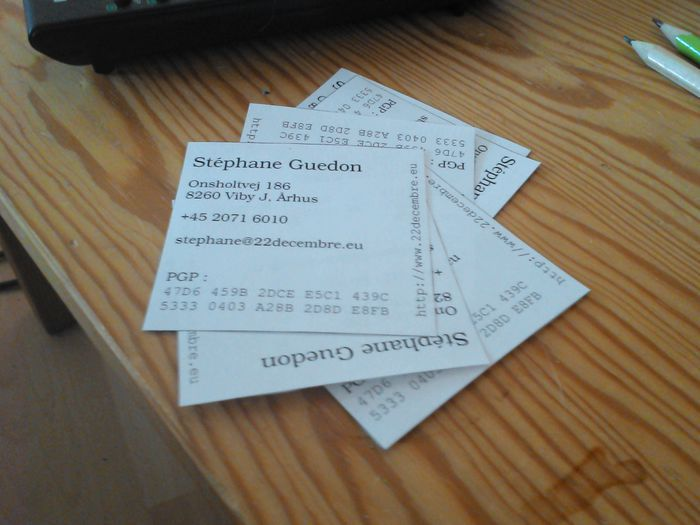
\includegraphics[width=\linewidth]{images/visiting.jpeg}
\caption[Des cartes de visites comportant une empreinte de clé GPG]{}
\end{figure}

Je suis toujours aussi surpris qu'après les
\href{http://fr.wikipedia.org/wiki/R\%C3\%A9v\%C3\%A9lations_d\%27Edward_Snowden}{révélations
d'Edward Snowden} sur la surveillance de masse des services secrets
américains (NSA, CIA\ldots{}), et les découvertes, chaque jour de
l'étendue et des \href{http://www.lemonde.fr/pixels/article/2015/02/17/un-nouveau-logiciel-espion-de-la-nsa-mis-au-jour_4577707_4408996.html}{pouvoirs}
des services secrets occidentaux - y compris français -, il y ait des
gens (la \emph{majorité} des gens en fait, aussi triste que ça puisse
paraître !) qui ne connaissent pas GPG !

Je me suis donc décidé à publier ce puis un tutoriel au long court qui j'espère, vous permettront d'apprendre à l'utiliser correctement.

\section{La démarche}\label{la-duxe9marche}

À l'opposé de la plupart des tutoriels que vous trouverez sur le net à
propos de GPG, je vais m'efforcer de vous donner les points importants
progressivement, de sorte que vous preniez le temps d'assimiler tout
cela.

En effet, il est inutile, si ce n'est dangereux de vous montrer comment
créer des clés de chiffrement, de vous mener par la main sur tout le
chemin et de vous lâcher dans la nature au bout, à peine deux jours
après vous avoir mis dans le bain.

Il vaut mieux être bien plus progressif. Vous faire réflechir et vous
donner les liens pour comprendre et vous permettre d'approfondir votre
apprentissage et votre compréhension.

\section{C'est quoi GPG ?}\label{cest-quoi-gpg}

\subsection{Tout d'abord il y eu PGP}\label{tout-dabord-il-y-eu-pgp}

PGP est un sigle pour \emph{Pretty Good Privacy}, \emph{Plutôt Bonne Vie Privée} en français.

PGP est le logiciel originel, conçu par \href{http://philzimmermann.com/FR/background/index.html}{Philip Zimmermann}, dans le
\href{http://openpgp.vie-privee.org/pourquoi.htm}{but explicite de
défendre la vie privée, les libertés individuelles et plus largement la
démocratie}.

C'est à la base un outil permettant de signer et chiffrer sa correspondance électronique. En français, son mail ou son courriel.

Ce mot, \emph{chiffrement}, il est très important : il indique que l'on
fait appel ici à des mathématiques de très haut niveau, avec des
concepts et des algorithmes complexes.\\Pas d'inquiétude toutefois !
C'est le logiciel lui-même qui fait ces opérations mathématiques.

\subsection{Puis OpenPGP}\label{puis-openpgp}

Puis l'IETF, a normalisé PGP et ça a donné le format de chiffrement
\href{https://fr.wikipedia.org/wiki/OpenPGP}{OpenPGP}, qui garantit que
les différents utilisateurs du format peuvent échanger grâce à ce même
format d'échanges.

\subsection{Finalement est venu GPG}\label{finalement-est-venu-gpg}

Ceci a permis à des développeurs libristes de concevoir un logiciel,
\href{https://www.gnupg.org/}{GnuPG}, abrégé en GPG, implémentant le
format OpenPGP.\\Autrement dit : grâce à OpenPGP, les utilisateurs de
GnuPG et PGP peuvent correspondre ensemble sans problème.

\section{Pourquoi l'utiliser ?}\label{pourquoi-lutiliser}

Vous êtes en couple ? Votre femme (ou votre homme \ldots{}) vous envoie
des photos osées pour vous exciter, ou plus simplement vous échangez des
propos classés X, que vous ne souhaiteriez surtout pas laisser à
disposition du premier venu !

Vous avez une compétition de cuisine et voulez partager votre recette de la tarte au citron avec Bree Hodges, mais pas avec Katherine Mayfair ?

Vous voulez monter une entreprise, ou vous travaillez déjà, et souhaiter donc communiquer en toute sécurité avec vos associés ?

Vous êtes \href{\{filename\}../nouveau-journalisme.md}{journaliste} et
voulez communiquer de manière sécurisée avec vos sources ?\\Ce cas est
particulier, puisqu'idéalement, vos sources doivent pouvoir, dès le
départ, sans même vous connaître, communiquer avec vous de manière
confidentielle !\\Il est à noter que ce fut le cas d'Edward Snowden : il
a utilisé PGP et demandé à ses contacts de faire de même pour assurer
des échanges sûrs.

Certaines de ces raisons semblent futiles.\\Mais ce que \emph{Desperate
Housewives}, et les gens autour de nous, nous ont bel et bien montré,
c'est que, aussi futile que ce soit, quelqu'un peut néanmoins être assez
motivé pour vouloir ouvrir votre courrier et dans ce cas, cette personne
mettra aussi en œuvre les moyens les plus importants, et parfois de
manière totalement disproportionnée.

Mais passons à autre chose\ldots{}
Ouuuuiiii\ldots{}\\

\href{http://www.linformaticien.com/actualites/id/32860/google-lit-vos-mails-et-assume.aspx}{Google},
\href{http://www.zdnet.fr/actualites/yahoo-lit-les-emails-de-ses-utilisateurs-quoi-de-neuf-doc-39791003.htm}{Yahoo}
et \href{https://tosdr.org/\#microsoft}{Microsoft} (Live et Hotmail par exemple) lisent vos courriels pour faire du profilage !

Vous rappelez-vous de ce scandale, avec des
\href{http://www.huffingtonpost.fr/2014/09/02/jennifer-lawrence-nue-piratage-internet-kate-upton-photos-celebgate_n_5745970.html}{photos
de stars de cinéma volées} ?\\Si vous estimez que la reaction de ces
stars (indignation devant les violations de leur vie privée) est
normale, saine, pourquoi n'accordez-vous pas la même valeur à votre vie
privée aussi ?

Bonne nouvelle toutefois,
\href{http://www.ginjfo.com/actualites/politique-et-economie/espionnage-nsa-depose-les-armes-devant-certaines-solutions-cryptage-20141230}{GPG
est toujours sûr apparament} !

D'ailleurs, pour vous donner une autre raison d'utiliser GPG : le mail,
à la base, c'est du texte. Rien de plus simple à intercepter, lire,
détourner. En fait, envoyer un mail, c'est envoyer une carte postale !

Ça va bien pour parler des photos du chat, mais très rapidement, ça
devient critique\ldots{} Non ?

\section{C'est douloureux ?}\label{cest-douloureux}

Disons que l'utilisation du chiffrement n'est pas forcement
hyper-simple. Toutefois, je ne vois aucun moyen, ni
\href{http://www.itespresso.fr/nsa-se-mobilise-casser-chiffrement-donnees-85704.html}{aucune
raison sérieuse} de s'en passer.

En mettant à disposition de tous un tutoriel perenne, en vous
permettant, progressivement, de découvrir le fonctionnement d'OpenPGP,
j'espère vous permettre et vous encourager à proteger votre vie privée
et vos libertés individuelles, et celles des personnes qui vous sont
chères.

Vous verrez qu'après un peu d'entrainement, l'utilisation de cet outil
devient très vite naturel.

\section{D'autres liens}\label{dautres-liens}

Jujusete (justement une journaliste) a écrit
\href{http://seteici.ondule.fr/2013/05/emails-sortez-couverts/}{cet article}.

Vous avez
\href{https://www.ted.com/talks/glenn_greenwald_why_privacy_matters}{ici}
une conférence en anglais de Glenn Greenwald, un des deux journalistes
ayant aidé Edward Snowden (décidément, on en voit beaucoup des
journalistes ici\ldots{} Qu'est-ce qu'ils ont tous avec ça ?).

\begin{quote}
Quand il y en a un ça va. C'est quand il y en a beaucoup qu'il y a des
problèmes.
\end{quote}

Il y a aussi \href{http://www.uzine.net/article128.html}{ceci}.

Et plein d'autres\ldots{}

	\chapter{Existe t-il des alternatives sérieuses à l'utilisation de GPG ?}

\emph{NB : Cet article est plutôt destiné aux personnes à compétences
techniques dans le domaine de l'informatique, communément appelées
}\textbf{geeks} ou \textbf{\emph{nerds}}. Toutefois les novices peuvent
y lire des choses intéressantes pour eux. Ils sont donc invités dans ce
cas à faire des recherches et à avoir beaucoup de patience dans
celles-ci.

On a donc OpenPGP et ses implémentations logicielles, PGP et GPG, des
outils pour protéger son courriels des regards indiscrèts. Mais est-ce
le meilleur moyen ?

\section{Bitmessage}\label{bitmessage}

Il existe par exemple Bitmessage
\footnote{\url{http://www.bortzmeyer.org/bitmessage.html}}, qui est
pour moi l'anti-exemple parfait, puisqu'il ne respecte pas le
paradoxe de la moquette\footnote{\url{http://www.22decembre.eu/2015/02/23/carpet-paradox-fr/}} : les adresses ressemblent furieusement à des chaînes de
caractères aléatoires, il n'est donc pas aisé de donner son adresse à son interlocuteur.

Même donner son adresse sur papier présente le risque que votre interlocuteur se trompe en la recopiant.\\Il n'est donc rien de plus
facile que de se gourer et d'envoyer son message à quelqu'un d'autre.\\Je pense que le moyen le plus efficace est encore de copier
son adresse sur un site web (et encore faut-il être prudent !).

La base du fonctionnement du réseau Bitmessage lui-même est compréhensible. Mais dès qu'on essaye de comprendre davantage
(essentiel, lorsqu'il s'agit de protocoles de sécurité et de chiffrement), on se met à se gratter la tête !

\subsection{Un petit truc étrange, une réflexion, comme ça\ldots{}}\label{un-petit-truc-uxe9trange-une-ruxe9flexion-comme-uxe7a}

Il y a également un truc qui me chiffonne, outre l'aspect obscur, non-écologique, non-efficient au plan énergétique : le protocole
Bitmessage est conçu pour noyer les communications chiffrées dans le flot des données P2P bit-torrent.\\Ainsi, soit disant, la NSA (qui est
typiquement l'organisme auquel les concepteurs du protocole tentent d'échapper) ne verrait pas ce flot de données.

Mais justement, la NSA a maintenant connaissance d'un protocole de communications sécurisé utilisé par des hackers de haut-niveau !\\Enfin
du moins, elle doit être au courant : elle lit des courriels, visite les sites web et les forums\ldots{}

On \emph{doit} assumer qu'elle est au courant ! Donc quelqu'un a conçu
un protocole de communications dans le but d'échapper à la NSA, et ce
protocole envoie en permanence \emph{tous} les messages à \emph{tout} le
réseau.

Quoi de plus facile pour la NSA (et pour tous les autres maintenant) de
se créer une ou plusieurs adresses Bitmessage, moissoner le flux
indistinctement, et tenter de casser le code de chiffrement,
puisqu'apparemment, c'est ce qu'elle fait déjà \footnote{\url{http://www.nytimes.com/2013/09/06/us/nsa-foils-much-internet-encryption.html} - lien en anglais} !

Le code de Bitmessage repose, en partie sur SSL/TLS, une technologie commune et répandue, sur laquelle tout le monde travaille. Pas le plus
sûr comme je l'indique plus bas.

\subsection{GPG ou Bitmessage ?}\label{gpg-ou-bitmessage}

\begin{notice}
Je précise que ceci est mon opinion, mon utilisation de mes outils informatiques. Ce n'est pas un commandement sacré à respecter au pied de
la lettre. Il peut y avoir débat. Si vous voulez troller, libre à vous, mais ce sera sans moi !
\end{notice}

Je préfère donc utiliser GPG plutôt que Bitmessage. Le courriel est
légitime, je n'ai pas de raison de le cacher - même si je comprends les
arguments de ceux qui le veulent, entre autre cacher \emph{à qui on écrit}.

Utiliser Bitmessage me marque automatiquement comme un \emph{hacker} de
haut vol, ce que je ne suis pas. Tout juste puis-je et souhaite
prétendre au status de \emph{petit} hacker ou de \emph{padawan}\ldots{}

En utilisant Bitmessage, j'encourage des gens à surveiller mon courriel
et à tenter de le lire.

Au contraire, en écrivant des courriels signés et/ou chiffrés, j'assume
ma correspondance, et en même temps je la protège, ce qui est on ne peut
plus légitime. Et comme c'est toujours du courriel, ça incite mes
contacts à utiliser GPG\ldots{}

Et si quelqu'un s'amuse à décrypter mon courriel, il découvrira alors
probablement mes échanges avec mon amie lesbienne ou mes propositions de
projets dans le cadre de mon travail. Des choses hautement inutiles pour
NSA \& co !

Point bonus : à moi, ça me m'a demandé aucun effort, alors que mon amie la NSA a gâché X heures de temps de calcul dessus !

\begin{quote}
Et faire chier les gens qu'on n'aime pas dès le matin, c'est vraiment gratifiant !
\end{quote}

\emph{Extrait de l'interview de Coreight par Cyrille Borne}
\footnote{\url{http://cyrille-borne.com/article47/du-berger-a-la-bergere-l-interview-de-coreight}}

\section{Les autres systèmes de chiffrement classiques}\label{les-autres-systuxe8mes-de-chiffrement-classiques}

On peut chiffrer et authentifier son courrier avec SSL/TLS, par le biais
du format S/Mime. Certaines entités fournissent des certificats personnels gratuitement.

C'est le cas de DanID qui fournit le système d'authentification NemID, permettant d'accéder aux sites bancaires et gouvernementaux danois. Les
certificats fournis par NemID sont valides pour signer et chiffrer du courrier, et s'authentifier sur certains sites web, notamment
DBA, le Bon Coin danois, mais pas pour sécuriser son site web - hélas.

En apparence, ces certificats sont donc une bonne chose pour sécuriser son courrier (les certificats de NemID sont un premier pas en avant vers
l'identité virtuelle des citoyens après tout). Mais SSL et TLS sont assez sujets à critiques dernièrement, et la NSA (et d'autres agences de
renseignement certainement) a déjà cassé nombre de ses algorithmes apparemment.

J'ai tendance à me mefier de plus en plus de TLS, en plus de son manque
d'ergonomie, parce qu'apparemment c'est aussi solide qu'une passoire en
plastique et tout aussi troué.

\begin{notice}
	Néamoins, je recommande toujours l'utilisation de TLS dans la navigation web ! Un bouclier en plastique, c'est mieux que pas de bouclier du tout !
\end{notice}

SSL/TLS et GPG sont toutefois deux implémentations légerement différentes du même principe : chiffrement asymétrique, avec une clé
publique et une clé privée. Dans les faits, ce n'est donc pas vraiment plus facile, et certainement pas plus sûr d'utiliser SSL/TLS.

Pour le courriel, je pense qu'il vaut mieux utiliser un outil conçu pour ça, à savoir GPG.

\section{Retour à GPG}\label{retour-uxe0-gpg}

GPG lui s'efforce de respecter le paradoxe de la moquette : il s'appuie sur des protocoles connus, assez bien maîtrisés et facile à prendre en
main (le courriel).\\Les clés peuvent être identifiées par l'adresse
courriel et/ou l'empreinte. Ceci permet de les trouver facilement et rassure les utilisateurs.

Et il n'était pas cassé par la NSA au dernières nouvelles.
	%\mainmatter
	\chapter{Installation des outils de base}

\section{Les logiciels nécessaires}\label{les-logiciels-nuxe9cessaires}

Pour pouvoir utiliser GPG, il vous faut \ldots{}

\begin{enumerate}
\def\labelenumi{\arabic{enumi}.}
\item GPG
\item Un gestionnaire de clés tel que :

  \begin{itemize}
  \item Kgpg/Kleopatra
  \item Enigmail
  \end{itemize}
  
\item Un client courriel tel que :

  \begin{itemize}
  \item Kmail
  \item Thunderbird
  \item Évolution
  \end{itemize}
\end{enumerate}

Très souvent, les gestionnaires de clés sont des logiciels additifs aux
clients courriels, des extensions. Ils ont pour la plupart les mêmes
options de base. Le choix de tel ou tel environnement s'avère donc
trivial, une affaire de goût et d'esthétique plutôt que de
fonctionnalités.

Kgpg est un élément de la suite KDE, qui s'utilise donc surtout avec
Kmail et Kontact. De même Enigmail fonctionne avec Thunderbird.

\begin{notice}
	Il est à noter que les tablettes et téléphones Samsung avec
Android ont maintenant tous les outils GPG nécessaires. Le problème
c'est que vous ne pouvez vraiment leur faire confiance.\\
\\
C'est néanmoins un bon moyen pour faire votre initiation à GPG.
Vous voudrez certainement recréer des clés après ça sur un vrai
ordinateur.
\end{notice}

Au passage, vous pouvez envisager, si vous êtes vraiment motivé,
d'installer votre propre système de courriel. Ça devient accessible au
non-informaticien, grâce à YunoHost \footnote{\url{https://yunohost.org/}} par
exemple. Ou dans une autre philosophie, OpenBSD, très simple
d'installation\footnote{\url{http://blog.chown.me/pourquoi-j-adore-openbsd.html}}, mais un poil difficile à prendre en main. Toutefois, pas plus difficile, de base, qu'une Debian.

\section{Recommandations}\label{recommandations}

\begin{notice}
La plupart de ces recommandations sont d'ordre général. Il s'agit de ce
qu'on pourrait appeler ``des pratiques de base saines pour votre
ordinateur''.
\end{notice}

\subsection{Sécurité du courriel}
En gros, il faut éviter le webmail, qui est une très mauvaise chose -
déjà de base - puisque vous accédez à votre courriel via le web, donc on
ne maîtrise pas la sécurité. Sans même parler d'utiliser GPG là dedans !

Le chiffrement et les signatures de vos courriels ne vous protégeront
nullement contre les virus et autres saloperies qui traînent ! Ils vous
garantiront que vos courriels sont bien authentiques et/ou n'ont pas été
lus par une autre personne que le destinataire légitime.

\subsection{Sécurité des logiciels}
Il faut également éviter de récupérer des logiciels sur des sites tiers
comme 01net et telecharger.com. Il est plutôt recommandé d'aller voir
le site web du concepteur du logiciel - tout en restant prudent\footnote{\url{http://cyrille-borne.com/article398/le-site-de-confiance-c-est-termine}}, ou un site officiel, comme le site web d'Apple pour le cas d'un logiciel pour Mac
par exemple.

Lorsque vous pouvez utiliser un logiciel libre ou open-source plutôt
qu'un logiciel propriétaire, faîtes le. C'est d'autant plus important
dans le cadre de protocoles critiques (sécurité\ldots{}). En effet,
avec un code en libre accès, n'importe qui peut vérifier la qualité du
code, garantir l'absence de portes dérobées, de pratiques douteuses. Un
code source ouvert (\emph{opensource}) signifie donc que vous pouvez lui
faire confiance pour \emph{vous protéger, vous et votre vie privée} ! Et
si vraiment vous êtes paranoïaque (c'est votre droit) alors vous pouvez
prendre des cours de code, puis faire vous même cette vérification !

Lors de l'installation d'un logiciel, ne faîtes pas «entrée» à tout va.
Regardez les options. Il est fréquent qu'un installateur vous propose
une barre d'outils ou autre, que vous n'avez pas demandé, et dont vous
n'avez pas besoin. Ces micro-ajouts permanents sont source de
ralentissements multiples, et contiennent parfois des logiciels espions.

Certains auteurs de logiciels signent leurs binaires (le fichier à
télécharger) avec leur clé gpg ou indiquent les sommes de contrôle MD5
ou SHA. Je ne vous ai pas encore expliqué comment vérifier les
signatures, mais si vous savez le faire, faîtes le !

\subsection{autres liens et documentations utiles}

SPF a écrit un guide pour la navigation internet plus sûre\footnote{\url{http://sanspseudofix.fr/kit-de-base-du-surf-tranquille-2/}}.
Genma (un fervent partisan de l'utilisation des outils de chiffrement) a son guide d'hygiène numérique\footnote{\url{http://genma.free.fr/?Petit-guide-d-hygiene-numerique}} \footnote{\url{https://github.com/genma/Conference_Guide_d_hygiene_numerique/blob/master/Genma_Petit_Guide_d_hygiene_numerique.pdf?raw=true}}.

\section{GPG}\label{gpg}

Comme je l'ai écris dans l'introduction, \emph{OpenPGP} est une norme décrivant le protocole, soit en fait l'ensemble de ce que doit faire le logiciel et ses composants (signatures, chiffrements, algorithmes, formats de messages…). \emph{GPG} ou \emph{GnuPG}, est un logiciel libre conçu suivant cette spécification.\\
\\
Je peux parler indifférement de clé \emph{GPG} ou \emph{OpenPGP}, puisqu'en l'occurence, les clés créées par \emph{GPG} doivent belles et bien correspondre au standard \emph{OpenPGP}.\\
\\
Sinon, quand j'utilise le terme \emph{OpenPGP}, je fais réference au protocole, donc, pour ce qui vous concerne, à la manière d'utiliser vos clés. Quand j'utilise \emph{GPG}, alors je parle du logiciel lui-même.

\subsection{Linux and co}\label{linux-and-co}

Gpg est dans les standards des distributions Linux. Si vous ne l'avez
pas, c'est que votre distro est tellement particulière que je n'en
connais pas le mode d'installation ou de gestion des paquets (
\emph{Slitaz} ?).

Sous Debian \& co, si c'est pas déjà installé - ce qui serait bizarre
puisque Debian utilise GPG pour signer et vérifier l'intégrité et
l'authenticité des paquetages logiciels (!) , ça donne ça :

\begin{lstlisting}
apt-get install gnupg gnupg2
\end{lstlisting}

J'indique les deux paquets. La version 2 est celle recommandée
aujourd'hui.

De toute façon, il est dans les dépendances de tous les gestionnaires de
clés qu'on verra plus loin.

Les utilisateurs d'autres distributions ou d'outils graphiques tels que
Synaptic, Apper ou Muom feront simplement une recherche sur
\textbf{gnupg}. Il y a de fortes chances que votre gestionnaire de
paquets vous dise qu'il est déjà installé.

Il est aussi dans la base des Unix tel qu'OpenBSD.

\subsection{Windows}\label{windows}

Bon, là on s'attaque à un gros morceau !

Il vous faut en fait Gpg4win \footnote{\url{http://www.gpg4win.org/download.html} - prenez la première version en haut, sauf si vous savez ce que vous
faîtes}, qui contient d'ailleurs tout le nécessaire\footnote{\url{http://www.gpg4win.org/about.html}}: gestionnaire de clés, client
courriel\ldots{}

Une fois l'installateur téléchargé, lancez le. Il vous proposera d'installer d'autres logiciels en plus de GPG.

\begin{itemize}
\itemsep1pt\parskip0pt\parsep0pt
\item
  GPA est un gestionnaire de clés
\item
  Kleopatra est un autre gestionnaire de clés
\end{itemize}

Vous avez besoin d'un des deux. Kleopatra est le plus décrit sur le web,
c'est donc celui que je conseille (et je l'ai sous la main, si vous me
demandez de l'aide, je pourrais plus facilement vous aider).

\begin{itemize}
\itemsep1pt\parskip0pt\parsep0pt
\item
  GpgOL, plugin pour Outlook
\item
  GpgEX, plugin pour l'explorateur de fichier de Windows.
\end{itemize}

Installez les si vous avez besoin.

\begin{itemize}
\itemsep1pt\parskip0pt\parsep0pt
\item
  Claws-Mail, logiciel de courrier léger
\end{itemize}

Les windowsiens, on vous facilite la vie décidément !

\subsection{MacOS}\label{macos}

Je n'ai pas de Mac sous la main. Mais Thunderbird est disponible sous
Mac et vous pouvez donc l'utiliser. Apparemment
le client courriel natif de Mac supporte également le chiffrement\footnote{\url{http://www.gbronner.net/mail/GPGMacOSX.html}}.

Vous avez besoin, des outils de chiffrements Gpg pour Mac. Téléchargez donc la suite
gpg\footnote{\url{https://gpgtools.org/}}.

Vous pouvez (bon en fait vous \emph{devriez}) vérifier l'intégrité du
fichier dmg en allant dans votre dossier de téléchargement (je suppose
ici qu'il s'appelle \emph{downloads} ) dans votre terminal :

\begin{lstlisting}
cd downloads
openssl sha1 GPG_Suite
\end{lstlisting}

En tapant le nom du fichier, vous pouvez après faire auto-complétion :
utilisez la touche de tabulation, le terminal complétera le nom du
fichier.

La commande ssl va vous indiquer une suite de caractères qui doivent
correspondre à celle indiquée sur le site de gpgtools en dessus du
bouton de téléchargement.

Reste plus qu'à installer. Ouvrez le fichier dmg et cochez ou décochez
les options qui vont bien.\\Il vous faut \emph{MacGPG2},
\emph{GPGPreferences}, \emph{GPG Keychain Access}.

Si vous utilisez le logiciel natif \textbf{Mail}, il vous faut aussi
\textbf{GPG for Mail}, mais si vous utilisez Thunderbird, il vous faut
par contre \textbf{GPG Services}.

\section{Un client couriel}\label{un-client-couriel}

\begin{notice}
Je ne décrirais pas la configuration de la messagerie, des adresses
courriels. Si vous êtes venus jusqu'ici, ce dont je vous félicite,
c'est que vous êtes motivés pour apprendre/chercher la solution par
vous-même et/ou que vous savez déjà configurer une adresse courriel.

Toutefois, on peut toujours me contacter\footnote{via l'adresse du tutoriel, ou aller sur \url{http://http://www.22decembre.eu/fr/contact.html}} pour demander de l'aide. Les tutoriels pour la configuration de la messagerie de Thunderbird (aisement transposable aux autres logiciels de courrier) sont légions sur le web.\footnote{\url{http://www.astucesinternet.com/modules/news/article.php?storyid=180} par exemple}.
\end{notice}

Bon, vous avez le logiciel de base installé, mais rien d'autre pour
l'instant à priori. Prenez le client courriel de votre choix.

\subsection{Thunderbird}\label{thunderbird}

Thunderbird est disponible en téléchargement et installation pour toutes
les plates-formes majeures\footnote{lien vers la page de téléchargement universelle: \url{https://www.mozilla.org/en-US/thunderbird/all.html}.
	Vous l'avez ici en français, et pour votre système: \url{https://www.mozilla.org/fr/thunderbird/}}.

Vous pouvez donc l'installer avec apt\footnote{Il est à noter que le logiciel est renommé Icedove sous Debian suite à la
	controverse entre Debian et Mozilla: \url{http://fr.wikipedia.org/wiki/Renommage_des_applications_de_Mozilla_par_Debian}} :

\begin{lstlisting}
apt-get install icedove
\end{lstlisting}

\subsection{Claws-Mail}\label{claws-mail}

Si vous êtes sous Windows, vous avez le client \textbf{Claws-Mail} dans
l'installateur de \textbf{Gpg4win}

\subsection{Kmail et Évolution}\label{kmail-et-uxe9volution}

Kmail est disponible comme partie de la distribution KDE, Évolution
comme partie de Gnome, donc si vous êtes sous GNU/Linux, vous devriez
utiliser votre gestionnaire de paquet favori.

\begin{lstlisting}
apt-get install kmail

apt-get install evolution
\end{lstlisting}

Même remarque qu'auparavant pour ce qui est des installateurs graphiques
: Synaptic et consorts installeront toutes les dépendances, y compris
\textbf{gnupg} si ce n'est pas encore le cas.

\subsection{Les autres}\label{les-autres}

Il existe une version Windows de KDE\footnote{\url{https://windows.kde.org/}},
mais je n'ai jamais pris le temps de l'essayer.

Sylpheed, client courriel disponible sous distributions Linux, Windows,
Mac et d'autres Unix.

\section{Un gestionnaire de clés}\label{un-gestionnaire-de-cluxe9s}

\begin{notice}
Rappel : Vous n'avez besoin que d'un seul de ces logiciels. Et très
souvent le choix de tel ou tel logiciel dépend de votre environnement !
\end{notice}

\subsection{GPG Keychain sous Mac OS}\label{gpg-keychain-sous-mac-os}

Le gestionnaire de clés s'appelle GPG Keychain sous Mac Os et vous
l'avez normalement déjà installé lorsque vous avez installé GPG pour
Mac.

\subsection{Thunderbird : Enigmail}\label{thunderbird-enigmail}

Si vous utilisez Thunderbird, vous avez besoin d'Énigmail, qui est en
fait une extension, un plugin du logiciel utilisé par Thunderbird pour
gérer son interaction avec GPG. Les utilisateurs de Thunderbird peuvent suivre le tutoriel du Hollandais Vollant
\footnote{\url{http://lehollandaisvolant.net/tuto/gpg/\#i2}}, qui est
complet et dont je m'inspire beaucoup. Toutefois je le trouve indigeste
car très long.

\subsubsection{Première solution : le site web}\label{premiuxe8re-solution-le-site-web}

L'installation est ici la même que pour l'installation d'un module
Firefox : xpi.\footnote{Il vous faut télécharger le plugin sur
\url{https://www.enigmail.net/download/} et bien sûr
prendre la version correspondant à votre OS.} 
Au passage, signalons comme l'indique bien
la page de traduction\footnote{\url{http://beta.babelzilla.org/projects/p/Enigmail/}} qu'Énigmail est traduit dans de nombreuses langues, y
compris français (90\%), mais pas danois, hélas.

L'extension xpi s'installe comme suit : il faut démarrer Thunderbird,
sélectionner «Outils» dans la barre des menus en haut, puis «plugins»,
«extensions» ou «modules».\\Ou alors (suivant votre version de
Thunderbird) cliquer sur le gros bouton en haut à droite, et
sélectionner «plugins», «extensions» ou «modules». Ici, vous pouvez indiquer à Thunderbird que vous souhaiter installer une
extension en cliquant en bas à gauche sur «installer\ldots{}».
Thunderbird vous demandera dans quel dossier de votre ordinateur vous
avez téléchargé le fichier xpi d'Énigmail.

Une fois cette opération réalisée, il faut redémarrer Thunderbird.

\subsubsection{Deuxième solution : télécharger via Thunderbird lui-même}\label{deuxiuxe8me-solution-tuxe9luxe9charger-via-thunderbird-lui-muxeame}

Vous pouvez demander à Thunderbird/Icedove de vous télécharger et
installer l'extension par lui-même. Allez dans la fenêtre des modules, comme indiqué précédemment et faîtes
une recherche sur Enigmail. Normalement vous devriez l'avoir en tête de
liste avec un bouton d'installation.

\subsubsection{Bonus Debian : installation via Apt}\label{bonus-debian-installation-via-apt}

Si vous utilisez Icedove (sic !) sous Debian, sachez qu'Énigmail est
dans les dépots Debian et que vous pouvez donc l'installer via apt.
C'est une bonne solution si vous partagez votre ordinateur avec d'autres
utilisateurs. Par contre, je pense que si on installe Énigmail par ce biais, il faut
alors éviter à tout prix de l'installer après par un autre moyen si vous
voulez mettre à jour. Si vous souhaitez une autre version que celle des dépots, il vous faut
la désinstaller au préalable.

\begin{warning}
Une seule version de ce logiciel par machine ! C'est, je
pense, une mesure de sécurité.
\end{warning}

\begin{lstlisting}
apt-get install enigmail
\end{lstlisting}

\begin{notice}NB : Il n'y a pas de raison, si Debian a inclus Énigmail dans ses
dépots que d'autres distributions GNU/Linux ne l'ai pas
fait\ldots{}\\Essayez donc de chercher Énigmail dans votre gestionnaire
de paquets.
\end{notice}

\subsection{Kgpg/Kleopatra}\label{kgpgkleopatra}

Kgpg et Kleopatra sont deux logiciels de gestion des clés et certificats
de chiffrement sous le bureau KDE. Pour ma part, je préfère me servir de
Kgpg, mais il est quand même très utile d'avoir les deux installés.

Il y a de fortes chances, si vous êtes un fan de KDE comme moi que ces
logiciels soient déjà installés. Mais sinon, comme précédemment, et
suivant votre distribution :

\begin{lstlisting}
apt-get install kgpg kleopatra
\end{lstlisting}

Rappelez-vous que Kleopatra est aussi distribué dans l'installateur
Gpg4win sous Windows.

\subsection{Les autres}\label{les-autres-1}

Il y a Seahorse sous Gnome, mais je ne connais pas du tout. Mais je
doute fortement qu'il soit très différent de Kgpg. Il est disponible
sous Debian :

\begin{lstlisting}
apt-get install seahorse
\end{lstlisting}

	\chapter{Un peu de théorie et de logique}

\section{OpenPGP, comment ça marche ?}\label{openpgp-comment-uxe7a-marche}

OpenPGP repose sur le principe de la cryptographie - ou chiffrement en français - asymétrique.

Quand on parle de clés GPG, on parle en fait de couples de clés : une clé publique et une clé privée.

\section{Pourquoi se compliquer la vie avec ça ?}\label{pourquoi-se-compliquer-la-vie-avec-uxe7a}

Lorsque vous signez un message, vous voulez garantir que celui-ci vient
bien de vous et qu'il n'a pas été altéré.\\C'est le même principe que
les sceaux au Moyen-Âge : le cachet de cire intact garantissait
l'authenticité et l'inviolabilité du message.

Vous devez donc signer votre message avec quelque chose que vous seul
avez en votre possession : votre clé \textbf{\emph{privée}} !

Et comment vos interlocuteurs vérifient-ils que ce message est
authentique ?\\Avec un élément qui est connu de tous, qui est public :
la vérification des signatures se fait avec votre clé
\textbf{\emph{publique}} !

Inversement, quand on chiffre un message à votre attention, on le rend
illisible pour toute personne n'en ayant pas la clé. Vous seul devez
pouvoir le lire avec quelque chose que vous seul avez en votre
possession : votre clé \textbf{\emph{privée}} !

Mais comme n'importe qui doit pouvoir vous envoyer des messages
chiffrés, l'opération de chiffrement doit se faire avec une information
connue de tous : votre clé \textbf{\emph{publique}} !

\section{Attention !}\label{attention}

Faîtes attention ! Un message signé \textbf{peut être lu par n'importe
qui sur le net}.

La signature garantit que vous êtes bien l'émetteur du message, et que
celui-ci n'a pas été altéré. Un message signé a donc plus de valeur
juridique qu'un message non signé.

\section{Récapitulatif}\label{ruxe9capitulatif}

On signe ses messages avec sa clé \emph{privée}. On vérifie
l'authenticité des messages d'autres personnes avec leur clé
\emph{publique}.

On chiffre les messages à destination d'autres personnes avec leur clé
\emph{publique}, qu'ils déchiffreront avec leur clé \emph{privée}.

Observez que c'est presque toujours le même côté de la liaison qui
utilise le même coté de la clé: vous utilisez presque toujours votre clé
privée, et vos correspondants n'utilisent que votre clé publique.

Votre clé privée doit donc être jalousement gardée et protégée !

%\begin{figure}[htbp]
%\centering
%\includegraphics{\{filename\}../images/gollum.jpg}
%\caption{}
%\end{figure}

C'est elle qui vous permet de contrôler votre coté de la liaison, de
prouver votre identité et de lire votre courrier !

VIendez lire l'article \href{\{filename\}4-key-generate-fr.md}{suivant}
où vous allez enfin créer votre clé GPG !

	\chapter{Générez et exportez vos clés GPG}

Let's go ! Vous allez faire votre première action concrète pour
l'utilisation de GPG : générer votre première clé !\\Ou plus exactement
votre première paire de clés, puisque rappelez vous : chaque clé GPG a
en fait une face privée et une face publique.

\textbf{Cet article peut sembler long ou ardu, mais il est important.
Créer les clés prend juste quelques minutes et vous n'avez quasiment
rien à faire. Donc s'il vous plait, prenez votre temps.}

\begin{notice}
S'il y a des gens inquiets: vous pouvez tout à fait utiliser une adresse
bidon pour ce tutoriel. Après tout, c'est bien ce que je fais avec
l'adresse du tuto.

Après cela, vous vous refaîtes des clés gpg avec votre vraie adresse, en
suivant à nouveau le tutoriel, mais vous ne les envoyez pas ici. Pas de
soucis !
\end{notice}

\section{Génération de la clé}\label{guxe9nuxe9ration-de-la-cluxe9}

Ouvrez votre gestionnaire de clés : Kgpg, Kleopatra ou Énigmail (ou un
autre encore\ldots{}) et chercher l'option de création de clés.

Sous Kleopatra, il s'agit de \textbf{\emph{Fichier \textgreater{}
Nouveau certificat \textgreater{} Créer une paire de clés personnelles
OpenPGP}}.

Sous Kgpg, il s'agit de \textbf{\emph{Clés \textgreater{} Générer une
paire de clés}}.

Sous Énigmail (donc dans Thunderbird lui-même), il s'agit de
\textbf{\emph{OpenPGP \textgreater{} Gestion de clés}}. Sélectionnez
alors \textbf{\emph{Générer \textgreater{} Nouvelle paire de clés.}}

\subsubsection{L'adresse à indiquer}\label{ladresse-uxe0-indiquer}

Le logiciel vous demandera quelle(s) adresse(s) vous voulez sécuriser
avec votre clé. Vous pouvez en effet mettre plusieurs adresses. Pour le
moment, c'est mieux de n'en mettre qu'une.

\subsubsection{Algorithme}\label{algorithme}

Il vous sera peut-être proposé plusieurs algorithmes : DSA \& ElGamal,
RSA \& RSA ou RSA.

Choisissez RSA \& RSA (dans Enigmail, onglet \emph{Avancé\ldots{}}, il
s'agit de l'option RSA). Il s'agit de la combinaison d'algorithmes la
plus forte et permet de chiffrer et signer.

\subsubsection{Longueur de clé}\label{longueur-de-cluxe9}

On vous demandera aussi la longueur de la clé à générer, avec ce choix :
1024, 2048 ou 4096 bits. Il y a peut-être d'autres choix, mais
globalement c'est ça.

Cette question indique en fait quelle sera la force de votre clé, sa
solidité, mais aussi le temps necessaire à la génération de la clé.

La longueur de clé choisie va demander au \emph{générateur de hasard} de
votre ordinateur une certaine quantité d'\emph{entropie}, quantité
exprimée avec ce nombre en \emph{bits}.

\begin{notice}
Je dois ici avouer ne pas comprendre vraiment le fondement profond de la
chose.\\Dès que j'essaye de comprendre ces concepts d'entropie, de
quantité d'entropie, je suis largué.\\En revanche, ce que je comprends
bien, c'est que plus il y a d'entropie, plus la clé est forte et le
chiffrement difficile à casser.
\end{notice}

Aujourd'hui, il est très recommandé de mettre 4096 bits. D'ailleurs je
pense que les prochaines versions des logiciels OpenPGP verront
apparaître des tailles de clés supérieures (puisque pour l'instant, 4096
est la limite) et/ou de nouveaux algorithmes.

La génération de la clé va prendre pas mal de temps. Il ne faut donc pas
s'inquiéter ou arreter votre logiciel précipitement.

Vous pouvez réduire ce temps en utilisant votre ordinateur. En effet,
plus vous utilisez votre ordinateur (particulièrement les accès
disques), plus vous générez l'entropie pour le générateur de
hasard.\\L'idéal, c'est donc d'en profiter pour mettre à jour sa
distribution (haute utilisation du disque dur) et d'aller jeter un coup
d'oeil sur la dernière vidéo de chaton sur vimeo\ldots{}

\subsubsection{Durée de validité}\label{duruxe9e-de-validituxe9}

On vous demandera normalement combien de temps la clé doit rester
valide.

Moi, ce que je fais, c'est que je donne une durée de validité d'un an,
que je repousse juste avant (un mois avant) l'échéance.\\Il s'agit ici
de ce qu'on appellerait un \emph{dispositif de l'homme mort} : si vous
veniez à perdre le contrôle de votre clé, celle-ci s'\emph{éteindra}
d'elle-même.

\subsubsection{Passphrase}\label{passphrase}

Il vous sera demandé une \textbf{\emph{passphrase}}. Une
\emph{passphrase} est un mot de passe très long. Donc par exemple quinze
ou vingt caractères.

Il existe plusieurs excellentes méthodes pour créer un bon mot de passe.

\begin{figure}[h]
\centering
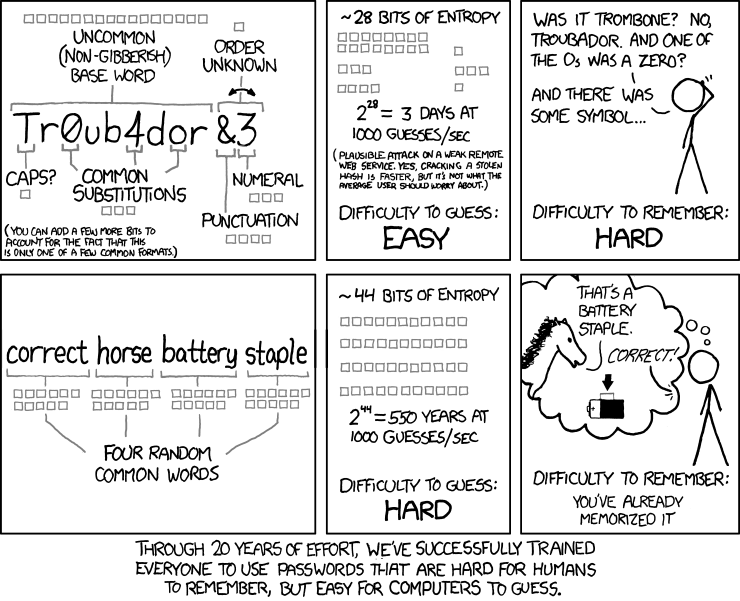
\includegraphics[width=\linewidth]{./images/password_strength.png}
\caption[Recommandations pour un mot de passe fort, par XKCD (https://xkcd.com/936/)]{}
\end{figure}

\emph{Bonus pour les profs de français ou les gens vivants en pays
étranger} :\\utilisez un mot compliqué, tel qu'un verbe particulièrement
ardu de la langue française à un temps de conjugaison improbable, et
hop, le mot de passe est presque impossible à trouver pour un humain
puisque peu de monde comprend votre langue, du moins à ce niveau.

Moi, ce que je fais, c'est que je prends un ou des mots de mon
environnement immédiat, ou un concept auquel je pense (en français, donc
j'ai déjà l'avantage indiqué au dessus).\\Puis je le \emph{tords}. Je
remplace le A par un À ou un @. Le L par ! ou autre chose du même genre.
J'ajoute des chiffres à un endroit choisi dans le mot.

Deux ou trois changements de cet acabit et le mot est méconnaissable et
donc difficile à deviner pour un humain, et un ordinateur (à cause de sa
longueur).

\subsubsection{De l'utilité de la passhprase}\label{de-lutilituxe9-de-la-passhprase}

Vous pouvez choisir de ne pas mettre de passhprase. Je dois avouer ne
pas l'avoir fait durant un long moment. Aujourd'hui je le fais et je le
recommande.

Ça ajoute tout simplement une sécurité supplémentaire. Chaque fois que
vous utiliserez votre clé, pour signer ou déchiffrer un message, ce mot
de passe vous sera demandé.\\Si vous n'êtes pas le seul à utiliser votre
ordinateur, ou si vous utilisez vos clés gpg sur votre tablette ou votre
smartphone (qu'on laisse fréquemment accessible sans le verrouiller),
alors vous avez intérêt à donner une passhprase.

\subsubsection{Certificat de revocation}\label{certificat-de-revocation}

Il est très probable que le gestionnaire de clé vous propose de générer
un certificat de révocation. C'est en effet une très bonne chose, donc
faîtes le s'il vous plait.

En cas de perte de la clé, de corruption, que quelqu'un entre en
possession de votre clé privée, hop, on publie ce certificat de
révocation sur les serveurs de clés. Très rapidement, par le jeu des
mises à jour mutuelles des serveurs, la clé est marquée comme invalide
sur l'ensemble du monde internet.

Ceci constitue donc une sécurité pour le cas où on vous volerait la clé
privée.

\emph{Si le logiciel ne vous propose pas la création d'un certificat de
révocation, ne vous en faîtes pas, je vous expliquerais la démarche en
détail dans un article futur.}

Si vous voulez changer de clé proprement, ce n'est absolument pas la
bonne méthode. Je vous en parlerais dans un autre article.

\section{Exercice}\label{exercice}

Comme j'ai pensé ce tutoriel comme pédagogique, je vais faire des petits
exercices ici et dans les articles suivants. Pour les besoins de ces
exercices, j'ai créée une adresse courriel sur mon serveur et des clés
pour cette adresse.

\textbf{\emph{Ces clés ne seront jamais utilisées pour une autre raison
que ce tutoriel.}}

Je vais vous demander en l'occurence d'exporter votre clé publique
fraichement générée, et de me l'envoyer en courriel, tout simplement.
C'est ce que beaucoup de personnes font pour échanger leurs clés.

Je vous renverrais alors un courriel où je vous dirais si votre clé a
les bonnes caractéristiques. J'ai également besoin de votre clé pour
l'exercice de l'article suivant.

\subsection{Exporter sa clé}\label{exporter-sa-cluxe9}

Pour m'envoyer votre clé, il vous faut l'\emph{exporter}.

Pour se faire, vous devez le demander à votre gestionnaire de clés.

Faîtes bien attention, votre gestionnaire de clés pourra vous proposer
d'exporter la paire de clés complète ou la clé privée.

Je parle bien, ici, de votre clé \textbf{publique} !

En effet, comme on l'a déjà signalé plus tot, et comme son nom l'indique
bien, la clé publique est à la disposition de tous.\\Le gestionnaire de
clé va vous proposer l'exportation de votre clé sous forme d'un fichier
d'extension gpg ou asc.

Ce fichier est en fait un bête fichier texte, qui contient la clé
publique, sous la forme d'une longue suite de caractères. Vous pouvez en
effet ouvrir le fichier avec Notepad ou un autre éditeur de texte par
exemple.

\emph{Et non, OpenOffice ou Word ne sont pas des éditeurs texte!}

\textbf{\emph{Toutefois, si vous ouvrez le fichier texte, ne le modifiez
surtout pas !}}

Vous pouvez alors me l'envoyer en pièce jointe d'un courriel à
\emph{Tuto-gpg @ 22decembre.eu}. Ni plus, ni moins.

\emph{NB : Kmail (client courriel de KDE), propose également dans son menu }\textbf{Joindre\ldots{}}* de mettre sa clé publique en pièce
jointe du courriel. Tout simple.

\section{D'autres liens}\label{dautres-liens}

Vous pouvez trouver d'autres conseils intéressants ici :

\href{https://securityinabox.org/fr/thunderbird_utiliserenigmail}{Security
in a Box}

\href{http://lehollandaisvolant.net/tuto/gpg/}{Le hollandais volant}

\href{https://help.riseup.net/fr/security/message-security/openpgp/gpg-best-practices}{Riseup}
	
	\chapter{Signer son courriel}

Vous avez suivi jusqu'ici et avez donc une clé gpg. Excellent !

Vous pouvez aussi demander de l'aide par courriel à l'adresse du
tutoriel : \emph{Tuto-gpg @ 22decembre.eu}.

On va maintenant faire en sorte que vous puissiez utiliser votre clé
dans votre courriel.

\section{Mais comment faire pour que vos divers contacts puissent utiliser votre clé ?}\label{mais-comment-faire-pour-que-vos-divers-contacts-puissent-utiliser-votre-cluxe9}

\subsection{Config' du client courriel}\label{config-du-client-courriel}

Déjà, il faut leur signaler l'existence de gpg.\\Un petit texte en bas
de votre courriel suffira. Ce texte est généralement appelé
\emph{signature}. Il faut bien le différencier de la signature par GPG
de vos messages.

Voici ma signature française par exemple :

\begin{quote}
Ce fichier \textbf{\emph{signature.asc}} ? C'est une signature GPG.\\Si
vous voulez savoir pourquoi j'utilise GPG et pourquoi vous le devriez
aussi, vous pouvez lire mon article
:\\http://www.22decembre.eu/2015/03/21/introduction-fr/
\end{quote}

Ce texte est à renseigner dans les options de votre client courriel.
C'est également là que vous indiquez vos options pour vos signatures
GPG.

\subsubsection{Kmail}\label{kmail}

Dans Kmail, c'est \textbf{\emph{Configuration \textgreater{} Configurer
Kmail \textgreater{} Identités}}.

Là, vous trouverez les options de chiffrement, où vous indiquez quelle
clé \textbf{\emph{privée}} vous utilisez pour signer vos messages. Vous
indiquez aussi ici quelle clé \textbf{\emph{publique}} est à utiliser
pour chiffrer les messages à destination de vous-même (excellent moyen
pour partager une info, un mot de passe entre plusieurs ordinateurs).

Sur la question du format, il
\href{http://blog.chown.me/choisir-pgp-mime-ou-pgp-inline.html}{vaut
mieux} utiliser le chiffrement \emph{OpenPGP/Mime}, plutôt que
\emph{inline}.

Il est également important d'indiquer vos préférences quand à la
rédaction des messages dans \textbf{\emph{Configuration \textgreater{}
Configurer Kmail \textgreater{} Sécurité \textgreater{} Rédaction}}.
Moi, j'ai presque tout coché (signer par défaut, chiffrer quand c'est
possible\ldots{}) sauf \emph{Toujours afficher les clés de chiffrement}.

\subsubsection{Thunderbird}\label{thunderbird}

Dans \textbf{\emph{Outils \textgreater{} Paramètres des comptes}},
sélectionnez le menu \emph{Sécurité OpenPGP} sous l'adresse qui vous
plaît. Cochez l'option \emph{Activer le support OpenPGP (Enigmail) pour
cette identité} ainsi que l'option \emph{Utiliser l'adresse électronique
de cette identité} pour identifier la clef OpenPGP.

Vous pouvez ensuite choisir vos options par défaut : chiffrer, signer
tous vos courriels ou non, et si vous voulez utiliser le format
\emph{PGP/Mime}, ce que je recommande (même remarque et même
\href{http://blog.chown.me/choisir-pgp-mime-ou-pgp-inline.html}{lien}
qu'au dessus).

Vous avez aussi des options à choisir dans \textbf{\emph{Enigmail
\textgreater{} Préférences}}.

\subsubsection{Évolution}\label{uxe9volution}

\emph{Édition \textgreater{} Préférences}

Dans la fenêtre dans l'onglet \emph{Comptes de messagerie}, puis le
compte en question et cliquer sur \emph{modifier}.\\Dans l'Editeur de
comptes qui s'ouvre, aller dans l'onglet \emph{Sécurité}.\\Dans le champ
\emph{ID de la clé PGP/GPG} : entrer l'identifiant en 8 caractères tel
que récupéré dans votre gestionnaire de clés.

Pensez aussi à mettre vos options par défaut.

Lors de la rédaction d'un nouveau message, dans le menu \emph{Options},
cliquer sur \emph{Chiffrer} ou \emph{Signer}.

\section{Faut-il signer et chiffrer tout son courriel ?}\label{faut-il-signer-et-chiffrer-tout-son-courriel}

La question est plus ou moins de nature philosophique et constitue un
choix personnel.\\De toute façon le logiciel de courriel a très
certainement de gros boutons qui n'attendent que d'être utilisés pour
réaliser ces opérations.

Pour ma part, j'aime bien cette remarque de Philip Zimmermann :

\begin{quote}
Que se passerait-il si tout le monde estimait que les citoyens honnêtes
devraient utiliser des cartes postales pour leur courrier? Si un
non-conformiste s'avisait alors d'imposer le respect de son intimité en
utilisant une enveloppe, cela attirerait la suspicion. Peut-être que les
autorités ouvriraient son courrier pour voir ce que cette personne
cache.\\Heureusement, nous ne vivons pas dans ce genre de société car
chacun protège la plupart de son courrier avec des enveloppes.\\Aussi
personne n'attire la suspicion en protégeant son intimité avec une
enveloppe. La sécurité vient du nombre.\\De la même manière, ce serait
excellent si tout le monde utilisait la cryptographie de manière
systématique pour tous ses e-mails, qu'ils soient innocents ou non, de
telle sorte que personne n'attirerait la suspicion en protégeant
l'intimité de ses e-mails par la cryptographie.\\Pensez à le faire comme
une forme de solidarité.
\end{quote}

Dans tous les cas, vous pouvez signer tous vos courriers sans que cela
pose de problème pour vos correspondants (normalement - il est possible
qu'ils en aient s'ils utilisent un mauvais client de messagerie. Mais
c'est extrêmement rare !).

\textbf{Un courriel signé est authentique. Votre correspondant aura la
certitude qu'il vient bien de vous et qu'il n'a pas été changé au cours
de son acheminement. En revanche, il n'est pas encore possible de
garantir que personne d'autre ne l'ait lû !}

En revanche, vous ne pouvez chiffrer vos courriers que si vos
correspondants utilisent eux aussi GPG ; puisque, rappelez-vous : vous
avez besoin de leur clé publique pour chiffrer des messages à leur
attention.

\section{Exercice}\label{exercice}

Bon, aujourd'hui, je vais vous demander de \emph{signer} un courriel à
mon intention. Tout simplement !

C'est pour cette raison que je vous ai demandé de m'envoyer la clé que
vous avez généré lors de la lecture du précédent article : j'en ai
besoin pour vérifier votre signature, donc pour vérifier que vous avez
bien compris cette partie du tutoriel.

Donc, revenons à l'exercice. Pour envoyer un courriel signé, ouvrez
votre logiciel de courriel, et écrivez un message à \emph{Tuto-gpg @
22decembre.eu}.

Vous pouvez écrire ce que vous souhaitez, y compris une critique du
tutoriel. Mais dans ce cas, j'aimerais qu'elle soit constructive,
qu'elle me permette de l'améliorer.

Avant de l'envoyer, sélectionnez \emph{Signer} dans les options ou
utiliser le bouton adéquat.\\Si (comme moi) vous avez demandé à votre
logiciel de courriel de signer tous vos messages, vous n'avez rien à
faire en fait ! Sauf appuyer sur le bouton \emph{Envoyer}\ldots{}

Quand vous aurez envoyé votre courriel, passez donc à
\href{\{filename\}6-crypted-mail-fr.md}{l'article suivant}.

Au plaisir de vous lire.

	\chapter{Lire et écrire du courrier chiffré}

Bon, j'ai dû vous envoyer un courriel chiffré. Donc lisible seulement
par vous.

\section{Ce que j'ai fais}\label{ce-que-jai-fais}

Lorsque j'ai récupéré votre clé publique, je l'ai mise dans mon
trousseau de clés.\\Ceci m'a permis de l'analyser, et donc de vous
indiquer que, oui, \emph{votre clé est bien générée}.

\section{Conséquences}\label{consuxe9quences}

Puisque j'ai votre clé publique, je peux désormais vous envoyer des
messages chiffrés.

\textbf{Avec un courriel chiffré, vous avez la certitude que vous seul
avez pu lire ce message. En revanche vous ne pouvez être sûr de
l'expéditeur.}

Par contre, si je signe également mes messages, vous ne pouvez pas
vérifier ma signature.\\En effet, encore une fois, pour vérifier ma
signature, vous avez besoin de ma clé publique, et je ne vous ai pas
encore indiqué comment la récupérer.

\textbf{La signature est une preuve d'authenticité du message, donc de
l'expéditeur.}

C'est pour cette raison que votre logiciel de courriel vous indique
sûrement que le courriel que je vous ai envoyé est signé par gpg, mais
qu'il ne peut en vérifier la signature.

\section{Un petit accroc}\label{un-petit-accroc}

Attention ! Seul le corps du message est chiffré ! Le sujet, l'en-tête
du message, ainsi que les méta-données (d'où le message a été envoyé, à
qui, et par où il est passé) sont en clair et lisibles de tous. Il est
difficile de faire autrement: comment les serveurs de messagerie
pourraient-ils savoir à qui remettre le message si la destination n'est
pas lisible ?

Il est donc recommandé de mettre un sujet assez neutre et générique si
vous voulez assurer une bonne confidentialité.

Quelque chose comme «Un bon plan» plutôt que «le plan de domination du
monde», ou «les derniers chiffres de production» plutôt que «chiffres de
prod' en hausse de 50 \%: on a tout bon !»

\section{Comment récupérer la clé publique ?}\label{comment-ruxe9cupuxe9rer-la-cluxe9-publique}

\subsection{Par courriel}\label{par-courriel}

J'aurais pu vous envoyer la clé publique du tutoriel, de la même façon
que vous m'avez envoyé la votre.

Mais ce n'est en fait pas très sûr: qu'est-ce qui garanti qu'une
personne malveillante n'a pas détourné votre courriel et remplacé votre
clé par une autre ?

C'est le genre de réflexions que je souhaite vous voir développer. La
sécurité sur internet est un processus, une manière de penser.

\subsection{Sur une page web}\label{sur-une-page-web}

Pour les personnes qui ont une page web, vous pouvez mettre votre clé à
disposition dessus. Il est de bon ton d'indiquer aussi l'empreinte de la
clé dans la page en question. Une empreinte de clé gpg est une suite de caractères alphanumériques
propre à chaque clé. Une empreinte permet donc à la fois d'identifier de
façon (relativement) sûre une clé et de garantir qu'elle est bien
intègre, que personne ne l'a corrompue.

Il est intéressant de voir qu'on utilise un vocabulaire réservé
d'habitude aux humains : \emph{intégrité} et \emph{corruption}. Il
s'agit bien d'indiquer des notions de confiance, d'absence de doute, de
probité.

Votre gestionnaire de clé vous donnera cette empreinte qui ressemblera à
ceci :

\begin{center}
\oldstylenums{30CF 1DA5 7E87 6BAA 730D E561 42E0 A02E F1C9 35A4}
\end{center}

Cette empreinte est celle de la clé publique de \emph{Tuto-gpg @
22decembre.eu}.\\C'est le même principe que les sommes de contrôle MD5\footnote{D'ailleurs les sommes de contrôle MD5 sont encore utilisées par OpenPGP, sauf que l'algorithme MD5 est aujourd'hui considéré comme obsolète. Le sujet sera évoqué dans la suite du tutoriel. Vous pouvez en apprendre davantage sur \url{http://fr.wikipedia.org/wiki/MD5}.} des
fichiers téléchargés sur internet - typiquement une iso de distribution Linux.

Certaines personnes mettent aussi l'empreinte de leur clé gpg sur leur
carte de visite, pour pouvoir les distribuer plus facilement.

\subsection{Les serveurs de clés}\label{les-serveurs-de-cluxe9s}

En connaissant une empreinte de clé gpg, on peut demander à son
gestionnaire de clés de trouver la clé sur internet ! En fait sur des
serveurs que l'on appelle «serveurs de clés» ou «serveurs gpg».

Voici quelques adresses de serveurs :

\begin{itemize}
\itemsep1pt\parskip0pt\parsep0pt
\item
  hkp://keyserver.ubuntu.com/
\item
  hkp://pool.sks-servers.net/ \footnote{Ce serveur est en fait un pool de serveurs de clés distribué par round-robind DNS. C'est le \textit{serveur} de clé le plus utilisé aujourd'hui.}.
\item
  hkp://pgp.mit.edu/
\item
  hkp(s)://keys.gnupg.net/
\end{itemize}

Vous pouvez indiquer à gpg d'utiliser en priorité le serveur que vous
préférez grâce à la configuration de votre gestionnaire de clés. Le S indique que vous pouvez utiliser ce serveur avec une connexion
sécurisée par TLS. L'avantage, si vous êtes parano, c'est que personne
ne sait quelles clés vous recherchez. L'intérêt de ces serveurs c'est de vous permettre de publier votre clé,
et de recevoir des clés et des messages signés et/ou chiffrés de la part
de personnes que vous ne connaissez pas.

\section{Exercice}\label{exercice}

En guise d'exercice aujourd'hui, je vais vous demander de récupérer la
clé publique du tutoriel, et de m'envoyer un courriel chiffré.

\subsection{Récupérer la clé
publique}\label{ruxe9cupuxe9rer-la-cluxe9-publique}

Vous l'avez compris, il s'agit de vous faire comprendre le
fonctionnement des serveurs de clés.

Pour se faire, vous devez ouvrir la boite de dialogue avec le serveur de
clé de votre gestionnaire de clés. Le logiciel vous proposera de faire
une recherche avec une chaîne de caractères. Autrement dit, une
empreinte, ou une adresse courriel. Soit vous copiez-collez l'empreinte de la clé du tutoriel (indiquée
juste au dessus) ou l'adresse courriel dans la boite de dialogue. Votre gestionnaire de clés va alors vous proposer une ou plusieurs clés
à télécharger.

Si vous avez indiqué l'adresse courriel, vérifiez que l'empreinte est
bien la bonne. Inversement, si vous avez indiqué l'empreinte, vérifiez
qu'il s'agit bien de la bonne adresse ! En effet, grâce à ces
empreintes, on peut vérifier que la clé que l'on a téléchargée est bien
celle qu'on cherchait.

Justement, j'ai créée plusieurs jeux de clés, non pas pour vous piéger,
mais pour vous faire réfléchir. Le but de ce tutoriel c'est de vous apprendre à utiliser GPG, donc il
vous faut l'utiliser pour le comprendre.

Au passage, vous pouvez noter que ces personnes ont signé cette clé:

\begin{itemize}
\itemsep1pt\parskip0pt\parsep0pt
\item
  \href{http://alterlibriste.free.fr/}{alterlibriste}
\item
  \href{http://lehollandaisvolant.net/}{le hollandais volant}
\end{itemize}

Je me suis en effet inspiré de leurs textes, ou ils m'ont encouragé à
écrire ce tutoriel. Je profite donc de ce moment pour les remercier,
ainsi que:

\begin{itemize}
\itemsep1pt\parskip0pt\parsep0pt
\item
  \href{http://genma.free.fr/}{genma}
\item
  \href{https://maymay.net/}{Maymay} qui m'a entre autre aidé avec
  quelques uns des articles anglais.
\end{itemize}

Regarder maintenant le courriel que je vous ai envoyé: votre logiciel
vous indique sûrement que la signature est valide, non ?

\subsection{Envoyer un courriel
chiffré}\label{envoyer-un-courriel-chiffruxe9}

Il faut donc que vous m'écriviez un courriel chiffré. Vous pouvez aussi
le signer, mais cela n'a pas d'incidence.

Juste avant de l'envoyer donc, cliquez sur le bouton \emph{Chiffrer} ou
selectionner l'option qui va bien. Voila !

Il est à noter que comme vous avez récupéré la clé publique du tutoriel,
il est très probable que votre logiciel de courriel vous ait proposé de
chiffrer le message lors de sa rédaction !

	\chapter{Signer des clés}

Je souhaite que vous puissiez commencer à utiliser activement gpg, au
moins avec des amis proches ou des membres de votre famille qui auraient
lu ce tutoriel, et pour cela, il faut que vous puissiez signer des clés.

\section{Signer des clés\ldots{}}\label{signer-des-cluxe9s}

Oui, avec gpg, on peut signer des courriels, des fichiers, mais aussi
des clés gpg !

\emph{Délicieusement récursif}

Lorsque vous signez une clé, vous accordez un certain crédit à celle-ci,
et vous l'indiquez également à tous ceux qui récupéreront votre
signature.

La signature d'une clé indique en fait que vous considérez que le
propriétaire de cette clé est bien légitime.

On va parler, là de \emph{cercle de confiance immédiat} (CCI pour
résumer): ce sont toutes les personnes que vous avez rencontré, dont
\textbf{vous} avez vérifié l'identité et signé la clé.

Retenez bien qu'il s'agit d'un concept que je définis ici, pour les
besoins de l'article, pour vous permettre de comprendre toutes les
notions ci dessous.

\section{Un problème d'identité}\label{un-probluxe8me-didentituxe9}

On va prendre un exemple: quelqu'un se présente pour faire signer sa
clé. Appelons le John.

Vous devez d'abord vérifier que John est bien le propriétaire de cette
clé, et pour se faire, vérifier avec lui l'empreinte de la clé.

Vous devez ensuite vérifier que John est bien qui il prétend être. Un
coup d'oeil (soigneux) à ses papiers d'identité vous le
confirmera\ldots{} mais pas seulement !\\Car l'identité, c'est bien plus
qu'un simple bout de carton plastifié, fut-il protégé avec des encres
spéciales\ldots{}

L'identité, c'est aussi les diverses fonctions qu'on occupe: trésorier
d'une association, blogueur plus ou moins anonyme, présence sur des
réseaux sociaux.

Tout ce qui renforce la confiance dans l'identité qu'une personne nous
indique peut être vérifié.

Une fois ces divers points validés, vous êtes à peu près sûr qu'il
s'agit bien de la bonne clé et de la bonne personne. Vous pouvez donc
signer sa clé.

\section{Confiance}\label{confiance}

En signant une clé, vous accordez également un certain niveau de
confiance dans son propriétaire.

Ce sont deux choses liées mais néanmoins distinctes, et il est important
de le comprendre.

Il y a cinq niveaux de confiance différents:

\begin{itemize}
\itemsep1pt\parskip0pt\parsep0pt
\item
  indéterminée/je ne sais pas (c'est le défaut)
\item
  absence de confiance/nulle
\item
  partielle
\item
  totale
\item
  absolue/c'est ma clé
\end{itemize}

Ce niveau de confiance traduit quelle confiance vous avez dans ce
propriétaire pour, lui-même, vérifier les identités et donc assurer son
cercle de confiance immédiat (CCI). Et ultimement, quelle confiance vous
accordez à son jugement à lui sur ceux d'autres personnes !

Par exemple, vous pouvez avoir vérifié soigneusement la clé d'un membre
de votre famille, un cousin mettons. Vous avez donc absolument confiance
dans \textbf{\emph{cette}} clé !

Mais par contre, vous pensez que votre cousin n'est pas encore bien rodé
avec OpenPGP. Peut-être qu'il signe un peu n'importe qui, ou qu'il
accorde une confiance excessive.

Vous n'avez donc aucune confiance dans son CCI.

Donc vous signez sa clé, mais avec une confiance nulle.

Et cette confiance nulle est quelque chose que vous pouvez (\emph{devez}
!) indiquer sans honte ni crainte. Pour ce faire, le niveau de confiance
est codé, inscrit dans la signature, de telle façon qu'il soit et reste
une information \emph{privée}.

\textbf{\emph{Vous êtes libre de votre jugement sur les gens dont vous
signez la clé ! Il s'agit là d'un cas de liberté d'expression et
d'opinion.}}

Plus vous respecterez ces diverses considérations, plus votre propre
jugement sera respecté par d'autres, en particulier des gens que vous
connaissez bien.

Et donc plus votre CCI prendra, lui une valeur haute également.

Pour ma part, je pense qu'on devrait signer avec une confiance partielle
par défaut, et réserver la confiance totale aux gens dont on connaît le
sérieux.

Votre CCI est donc à la fois constitué des clés (et donc de leurs
propriétaires) que vous avez signées, mais également du niveau de
confiance qui leur est accordé !

\section{Des exemples}\label{des-exemples}

Vous rencontrez quelques personnes dans un bar lors d'un rendez-vous de
votre LUG.

\subsection{Arthur}\label{arthur}

Arthur vous explique qu'il débute dans l'utilisation de GPG et souhaite
donc se construire une toile de confiance. \emph{Ok}.\\Vous vérifiez
correctement son identité et il fait de même avec vous. Puis, chez vous,
vous signez sa clé, puisque vous l'avez vérifiée.

En revanche vous lui accordez une confiance nulle, car vous estimez que
sa pratique de Gpg est encore trop récente.

Cette confiance nulle ne vous empêche pas, un mois plus tard, lors d'une
autre rencontre, de lui demander comment il gère son trousseau de clé,
de constater son sérieux et d'élever son niveau de confiance.

Cette confiance nulle n'empêche pas non plus cette personne de vous
accorder un jugement haut ou bas également.\\Et les signatures d'autres
personnes sur sa clé s'ajoute à la votre. Signatures peut-être plus
positives !

\emph{Il ne faut pas que vous vous sentiez honteux ou irrespectueux
d'indiquer une confiance basse à Arthur.}

\subsection{Miriam}\label{miriam}

Miriam vous explique qu'elle est développeuse Debian. Vous vérifiez son
identité et sa clé.\\Chez vous, vous vérifiez également ses dires au
sujet de Debian et vous constatez qu'elle a bien dit la vérité.

Donc vous signez sa clé, et vous lui accordez une confiance totale car
vous savez que les dev' Debian utilisent beaucoup GPG et doivent
respecter un certain sérieux.

\subsection{Greg}\label{greg}

Greg vous indique qu'il utilise très régulièrement Gpg. Après avoir
vérifié sa clé, vous la signez, avec une confiance
partielle.\\Simplement parce que vous ne le connaissez pas, mais vous
voyez Greg comme quelqu'un de sérieux. Sans plus.

\subsection{Karolina}\label{karolina}

Karolina vous explique qu'elle a adopté un système de signature très
précis décrit avec beaucoup de détails dans un document disponible sur
son blog (on parle là de \emph{politique de signatures}).

Vous trouvez sa démarche très juste et décidez de lui accorder une
confiance totale, précisément à cause de ce système de signatures dont
vous estimez le fonctionnement très équilibré.

\section{La Toile de confiance}\label{la-toile-de-confiance}

C'est quoi la toile de confiance (les anglophones parlent de \emph{Web
of Trust}) ?

La toile de confiance, ce sont tous les CCI additionnés et mis bout à
bout, constituant des chaînes:

Vous avez mis une confiance partielle en Greg. Donc son CCI se retrouve
lui aussi avec une confiance partielle.

Vous avez mis une confiance complète en Miriam. C'est comme si vous
aviez fait entrer tous ses contacts dans votre cercle de confiance à
vous.\\Et c'est Miriam qui a défini si oui ou non vous pouvez faire
confiance dans telle ou telle personne que vous n'avez jamais rencontré
- puisque vous avez confiance dans le jugement de Miriam.\\Si, donc,
elle a mis elle-même quelqu'un d'autre en confiance totale, alors cette
troisième se retrouve à nouveau \emph{de facto} dans votre cercle de
confiance \emph{étendu}.

Seulement, et c'est bien important, il ne \emph{faut pas que
}\textbf{vous}* signiez* une des clés signées par Miriam sans avoir
rencontré la/le propriétaire de cette clé.\\Miriam l'a fait. Donc la clé
qu'elle a signée sera reconnue comme valide par votre gestionnaire de
clés.\\D'ailleurs pourquoi signeriez vous une clé sans avoir rencontré
la personne ?

Gpg va déterminer par un algorithme jusqu'à quel point vous pouvez faire
confiance à telle clé, que vous n'avez pas signé, à travers le mécanisme
de la toile de confiance.

Par défaut, Gpg n'ira pas plus loin que cinq cercles de confiance. Et il
faut trois signatures avec une confiance partielle, ou une signature
avec une confiance complète pour qu'une clé soit valide.

\subsection{Corollaires}\label{corollaires}

Il faut se rendre compte également que la Toile de confiance doit être
considérée avec sérieux.

Par exemple, les opinions politiques, religieuses, son origine, son
sexe, sa couleur de peau ni même votre proximité sentimentale (ami,
membre de la famille\ldots{}) avec le propriétaire de la clé n'ont rien
à voir ici.\\Seul compte le sérieux qu'il accorde à son CCI.

Si vous rencontrez quelqu'un qui vous explique qu'il signe des gens
d'une manière très précise, avec une politique de signature détaillée,
vous pouvez être admiratif de son sérieux et décider de lui accorder une
confiance totale.\\Puis au cours de la discussion, vous vous rendez
compte que c'est un pédophile néonazi pronnant l'eugénisme et mangeant
des chatons au petit-déjeuner avec de la sauce soja, vous \emph{devriez
quand même} signer sa clé !

%\href{http://giphy.com/gifs/cat-black-and-white-food-S4IWCPAjhbzUc}{\includegraphics{http://i.giphy.com/S4IWCPAjhbzUc.gif}}

Bien sûr, vous le dénoncer à la police aussi sec, mais les deux actions
sont compatibles.

\subsection{Quelle est ma responsabilité dans tout ça ?}\label{quelle-est-ma-responsabilituxe9-dans-tout-uxe7a}

Il s'agit donc bien d'un système, d'un réseau de confiance
\emph{relative}.

Il n'y a pas d'autorité centrale de type étatique qui indique quelle
identité est vraie ou fausse.

C'est vous qui devez estimer quelle confiance vous accordez et à qui
vous l'accordez.

Ne soyez toutefois pas effrayé d'une telle responsabilité !

Le fonctionnement du réseau est démocratique: si vous attribuez un
mauvais degré de confiance à un utilisateur, votre ``vote'' sera
contrebalancé par ceux des autres.

Les \emph{politiques de signature} documentées et accessibles en ligne
renforcent cet aspect démocratique, parce qu'elles sont impartiales,
comme décrit au dessus (cf le néonazi mangeur de chatons).

%\href{https://www.flickr.com/photos/jmtimages/3286566742/}{\includegraphics{https://farm4.staticflickr.com/3615/3286566742_c673e4845d_z.jpg}}

La responsabilité est donc individuelle et distribuée. C'est en fait du
pair-à-pair ! C'est nous tous qui, collectivement, sommes l'autorité en
laquelle nous faisons confiance pour valider les clés.

\section{Tromperies ?}\label{tromperies}

\subsection{Que faire si quelqu'un tente de me tromper en me faisant
signer une fausse clé
?}\label{que-faire-si-quelquun-tente-de-me-tromper-en-me-faisant-signer-une-fausse-cluxe9}

Déjà, il faut bien voir qu'en signant une clé, vous validez aussi une
adresse courriel. Donc c'est aussi l'adresse courriel qu'il s'agit de
vérifier.

Et le plus simple dans ce cas est que la personne vous envoie un
courriel signé depuis cette adresse. (Il peut le faire quelques heures
plus tard, ce n'est pas un soucis).\\De cette façon, vous êtes sûr que
vous signiez la clé associée à cette adresse courriel, et qu'elle
appartient à la personne que vous avez rencontré.

C'est toutefois un poil lourd comme procédure. À vous de voir.

\subsection{Il peut arriver qu'on veuille écrire à quelqu'un qu'on ne
connaît pas ! Comment être sûr qu'on récupère la bonne clé
?}\label{il-peut-arriver-quon-veuille-uxe9crire-uxe0-quelquun-quon-ne-connauxeet-pas-comment-uxeatre-suxfbr-quon-ruxe9cupuxe8re-la-bonne-cluxe9}

C'est le rôle de la toile de confiance, décrite au dessus.

Si vous souhaitez écrire à Valentina, et que des gens mal-intentionnés
ont crée une ou des fausse(s) clé(s) qu'ils ont envoyés sur les serveurs
de clés, comment reconnaître la bonne ?

Il y a de fortes chances que la clé de Valentina soit celle qui comporte
le plus de signatures.\\Et, très important, plus ces signatures viennent
de personnes diverses (de nationalités, de fonctions diverses\ldots{}),
plus la clé sera sûre !

Il est par exemple très facile de créer des clés avec vingt signatures
dessus.

Il est par contre assez difficile de créer une clé avec une ou deux
\emph{fausses} signatures de dev' Debian. Or il est très facile
d'obtenir la signature d'un dev' Debian!\\Non pas que ce soient des gars
ou des filles \emph{faciles}. Mais ils sont nombreux et éparpillés un
peu partout.\\Si vous habitez une grande ville occidentale, il est
probable que vous ayez \emph{un dev' Debian à portée de main} et qu'il
signera votre clé (en suivant sa politique de signature) si vous
l'invitez pour une bière dans un bar.

S'il est donc facile de créer des clés avec de fausses signatures, il
est tout aussi facile de faire signer sa clé par une personne publique à
l'identité vérifiable (dev' Debian ou dev' d'autres logiciels libres,
blogueur, membre d'une association\ldots{}).

Et c'est donc cette dernière clé que vous utiliserez en cas de doute !

\section{Exercice}\label{exercice}

Bon, c'est bon, vous pigez le truc de la toile de confiance ?

Ne vous inquiétez pas, vous aurez d'autres articles qui donneront
d'autres détails. Et vous pouvez toujours revenir ici lire encore et
encore cet article.

Je vais vous demander pour l'exercice du jour, de signer la clé du
tutoriel, d'y mettre la confiance qui vous paraît correcte, puis de me
l'envoyer par courriel.

Nous sommes bien d'accord qu'il ne faut pas faire cela normalement,
puisque qu'on ne s'est pas rencontré.

C'est la raison pour laquelle j'ai indiqué dans un des articles que la
clé du tutoriel ne sera utilisée que pour les besoins du tutoriel.

\subsection{Donc, comment qu'on fait ?}\label{donc-comment-quon-fait}

Dans votre gestionnaire de clés, vous devez sélectionner la clé en
question, puis l'option \textbf{\emph{Signer}}.

Le logiciel vous demandera quelle confiance vous souhaitez accorder à
cette clé. Si vous avez plusieurs clés privées, il vous sera demandé
avec laquelle vous souhaitez signer.

Vous pouvez également passer par l'édition des propriétés de la clé et
changer simplement le niveau de confiance. La signature sera alors faîte
automatiquement.

Vous exportez ensuite la clé dans un fichier, que vous envoyez en pièce
jointe de courriel à \emph{Tuto-gpg @ 22decembre.eu}. Lorsque je vais
récuperer la clé, les signatures vont s'additionner les unes les autres.
Je vais alors vous répondre et vous envoyer votre clé, signée avec la
clé du tutoriel.

Summum de la feignantise, KGpg et d'autres logiciels vous proposent de
faire le tout s'un seul coup: avec l'option \textbf{\emph{Signer et
envoyer par courrier electronique}}, KGpg va effectivement signer
suivant vos directives, puis préparer le courriel avec la clé dedans.

\subsection{Précisions}\label{pruxe9cisions}

Certains logiciels (notamment KGpg) mettent l'accent sur la vérification
de l'identité du propriétaire de la clé pour vous indiquer le niveau de
confiance que vous pouvez accordez.

Il s'agit là en fait d'une assertion selon laquelle, puisque l'identité
et la clé ont bien été validées sérieusement, il est raisonnable de
penser que le propriétaire de la clé accorde le même sérieux dans
d'autres signatures.

Ceci ne change pas la signification de votre signature et ma description
reste valable: la confiance accordée indique à quel point vous estimez
le propriétaire de la clé capable d'entretenir son CCI.

C'est donc ce niveau de confiance que vous devez indiquer.

Ces logiciels ont par exemple une ergonomie trompeuse. Si vous avez des
questions, n'hésitez pas à lire et relire cet article ou à m'écrire.

\subsection{Inspirations diverses}\label{inspirations-diverses}

Vous pourrez trouver:

Le blog de \href{http://www.miriamruiz.es/}{Miriam Ruiz}, développeuse
Debian, dont j'ai utilisé le nom dans cet article.

\href{http://matrix.samizdat.net/crypto/gpg_intro/gpg-intro-5.html}{Samizdat}
et
\href{http://www.amula.asso.fr/site/article.php?id_article=80}{l'Amula}
qui m'ont parmi de comprendre le concept de Toile de confiance, et
aujourd'hui m'ont fourni une bonne base pour ordonner mes idées et donc
écrire le présent article.

	
	\chapter{Inspirations diverses}
	
	\begin{description}
		\item[Conférence TED en anglais de Glenn Greenwald, un des deux journalistes ayant aidé Edward Snowden:] \url{https://www.ted.com/talks/glenn_greenwald_why_privacy_matters}
			
		\item[Jujusete, une journaliste:]\url{http://seteici.ondule.fr/2013/05/emails-sortez-couverts/}\\
		
			
		Décidément, on en voit beaucoup des journalistes ici\ldots{} Qu'est-ce qu'ils ont tous avec ça ?
		
		
		\begin{quoting}	
		Quand il y en a un ça va. C'est quand il y en a beaucoup qu'il y a des problèmes.
		\end{quoting}

		%\begin{quote}
			
		%\end{quote}
		
		\item[Pourquoi j’utilise OpenPGP, par Jean-Marc Manach] \url{http://www.uzine.net/article128.html}
		
		\item[Security in a Box:]\url{https://securityinabox.org/fr/thunderbird_utiliserenigmail}
		
		\item[Le tutoriel du hollandais volant, qui m'a beaucoup inspiré:]\url{http://lehollandaisvolant.net/tuto/gpg/}
		
		\item[Les bonnes pratiques de Gpg et OpenPGP:]\url{https://help.riseup.net/fr/security/message-security/openpgp/gpg-best-practices}
		
		\item[Le blog de Miriam Ruiz, développeuse Debian, dont j'ai utilisé le nom dans l'article sur la signature des clés:]\url{http://www.miriamruiz.es/}\\
		
		
		
		\item[Samizdat:]\url{http://matrix.samizdat.net/crypto/gpg_intro/gpg-intro-5.html}
		
		\item[et l'Amula:]\url{http://www.amula.asso.fr/site/article.php?id_article=80}
		
		qui m'ont parmi de comprendre le concept de Toile de confiance.		
	\end{description}

	
	
	
\end{document}